\documentclass[10pt]{article}

\usepackage[paperwidth=19.2in,paperheight=10.8in,margin=0.45in]{geometry}
\usepackage{multicol}
\usepackage{amsmath,amssymb}
\usepackage{booktabs}
\usepackage[table]{xcolor}
\usepackage{tcolorbox}
\tcbuselibrary{skins}  % needed for 'title style'
\usepackage{graphicx}
\usepackage{array}
\usepackage{hyperref}
\usepackage{eso-pic}

\pagestyle{empty}
\setlength{\parindent}{0pt}
\setlength{\columnsep}{0.35in}

\definecolor{primary}{RGB}{0,150,255}
\definecolor{lightblue}{RGB}{235,245,255}

\tcbset{
    colback=white,
    colframe=primary,
    boxrule=1.1pt,
    arc=2mm,
    left=2mm,
    right=2mm,
    top=1mm,
    bottom=1mm,
    before skip=2mm,
    after skip=2mm,
    title style={fill=primary},
    coltitle=white,
    fonttitle=\bfseries\large
}




\begin{document}

\AddToShipoutPictureFG*{
  \AtPageLowerLeft{
    \raisebox{0.45in}{
      \makebox[\paperwidth]{
    \quad Barnab\'as Sz\'ekely \quad | \quad PhD Candidate, Goethe University Frankfurt \quad | \quad
\href{mailto:szekely@econ.uni-frankfurt.de}{szekely@econ.uni-frankfurt.de}
      }
    }
  }
}

{\centering
{\fontsize{34}{38}\selectfont \textbf{Bankruptcy Resolution and the Macroeconomics of Cash Flow-Based Lending}}\\[0.20in]
{\fontsize{18}{20}\selectfont Barnab\'as Sz\'ekely \hspace{0.3in}}\\[0.35in]
}

\begin{multicols}{3}

% ======================================================
% COLUMN 1: MOTIVATION, RQ, WHAT I DO
% ======================================================

\begin{tcolorbox}[title=Motivation]
Financial distress is a common event in a firm's life.
\begin{itemize}
    \item In each quarter $\sim$5.5\% of U.S. small and middle-market firms face financial distress     
    \item How firms resolve these episodes directly affects their access to credit
\end{itemize} \vspace{3mm}

Small and middle-market firms are often forced to shut down in default 
\begin{itemize}
    \item Due to the large costs of restructuring debt
    \item Small firms cannot credibly pledge future earnings as collateral
    \item This widens the financing gap between small and large firms
\end{itemize}
\vspace{3mm}

\textbf{Research Questions}
\begin{itemize}
    \item[1.] How do reorganization costs limit `small' firms' access to cash flow-based debt?
    \item[2.] How does this affect firm dynamics and aggregate outcomes?
\end{itemize}
\end{tcolorbox}

\begin{tcolorbox}[title=Empirical Motivation]
Cash flow-based debt is expensive for smaller firms.

\vspace{1.25mm}

\small
\begin{minipage}{0.21\textwidth}
    \centering
    \vspace{5mm}
    \textbf{Credit Spread:}
\end{minipage}
\begin{minipage}{0.56\textwidth}
    \centering
    \begin{tabular}{lcc}
        \toprule
        Total Assets & \textbf{$\leq$ 100M} & \textbf{$>$ 100M} \\
        \midrule
        Cash flow-based debt & 7.19\% & 3.12\% \\
        Asset-based debt & 5.25\% & 3.93\% \\
        \bottomrule
    \end{tabular}
\end{minipage}
\normalsize

\vspace{3mm}
\normalsize

\raggedright
Liquidation risk is substantial for smaller firms

\vspace{1.25mm}

\small
\begin{minipage}{0.20\textwidth}
    \centering
    \vspace{3mm}
    \textbf{Liquidation Risk:}
\end{minipage}
\begin{minipage}{0.56\textwidth}
    \centering
    \begin{tabular}{lcc}
        \toprule
        Total Assets & \textbf{$\leq$ 100M} & \textbf{$>$ 100M} \\
        \midrule
        Share Liquidated & 76.7\% & 7.61\% \\
        \bottomrule
    \end{tabular}
\end{minipage}
\normalsize


\normalsize
\end{tcolorbox}

\begin{tcolorbox}[title=What I Do]
I build a quantitative GE model featuring:
\begin{itemize}
    \item Representative household, competitive lender, and bankruptcy courts
    \item Heterogeneous firms with endogenous entry, exit, and default
    \item Financing under credit frictions: \textbf{asset-backed} and \textbf{cash flow-backed} borrowing
    \item Bankruptcy resolution through \textbf{liquidation} or \textbf{reorganization}
\end{itemize}


\vspace{4mm}

I use the model to study policy reforms that streamline reorganization.
\begin{itemize}
    \item Reducing reorganization costs lowers liquidation risk and narrows financing gaps
    \item Targeted reforms raise productivity by improving credit allocation and firm entry
\end{itemize}

\vspace{2mm}

\textbf{Policy implication:} facilitating reorganization improves credit allocation and productivity.
\end{tcolorbox}


\columnbreak

% ======================================================
% COLUMN 2: INTERMEDIATION, MECHANISM, MODEL FIT
% ======================================================

\begin{tcolorbox}[title=Financial Intermediation Process]

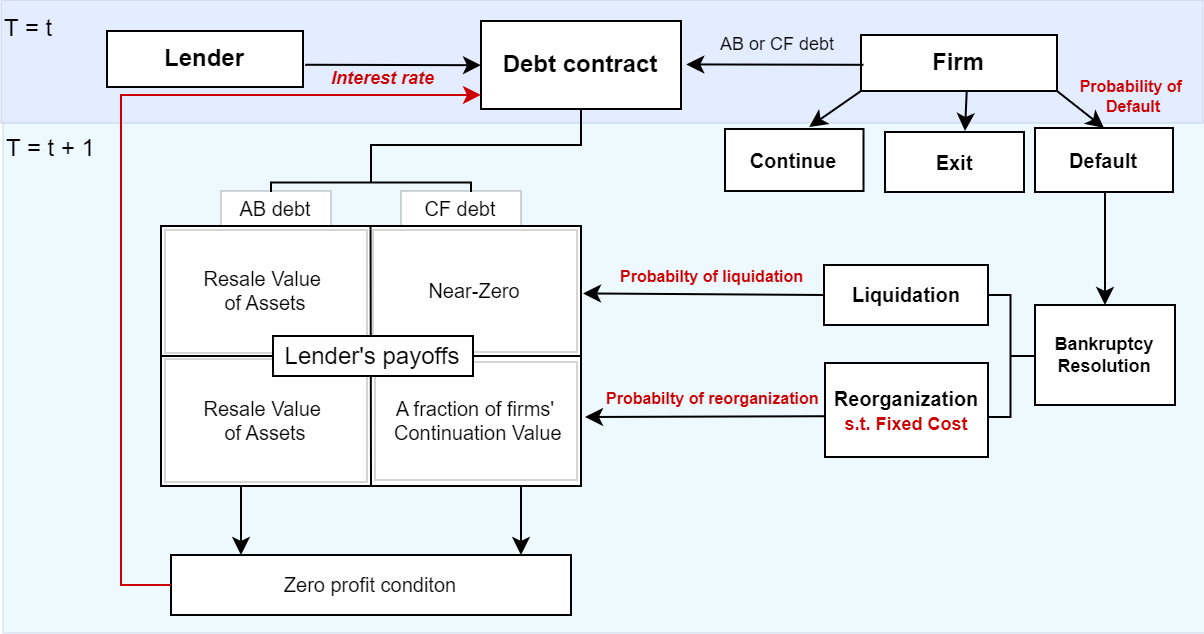
\includegraphics[width=1\textwidth]{Plots/min60_t7_fc.png}

\vspace{2mm}

\textbf{Model Mechanism:}
\begin{enumerate}
    \item Fixed reorganization costs make liquidation more likely for small firms
    \item Liquidation destroys future cash flows
    \item Cash flow-based lending to smaller firms is risky (see: near-zero recovery)
    \item Lenders charge higher spreads for smaller firms
    \item \textbf{Productivity Loss:} small, but productive firms operate below efficient scale
\end{enumerate}


\end{tcolorbox}

\begin{tcolorbox}[title=Model Fit]

The model is calibrated to U.S. non-financial corporations, 2010--2024. \vspace{2mm}

\small
\centering
\begin{tabular}{l|cc||cc}
& \multicolumn{2}{c||}{\textbf{Targeted}} & \multicolumn{2}{c}{\textbf{Untargeted}} \\
\toprule
\textbf{Moment} & \textbf{Target} & \textbf{Model} & \textbf{Small} & \textbf{Large} \\
\midrule
Liquidation prob. & 0.58 & \textcolor{red}{0.56} & 0.84 -- \textcolor{red}{0.85} & 0.20 -- \textcolor{red}{0.14} \\
Debt/Coll. & 0.52 & \textcolor{red}{0.50} & 0.44 -- \textcolor{red}{0.45} & 0.59 -- \textcolor{red}{0.57} \\
Interest rate & 5.36 & \textcolor{red}{5.30} & 5.89 -- \textcolor{red}{5.63} & 4.63 -- \textcolor{red}{4.89} \\
CF-reliance & 0.51 & \textcolor{red}{0.53} & 0.51 -- \textcolor{red}{0.24} & 0.53 -- \textcolor{red}{0.97} \\
CF debt/total debt & 0.82 & \textcolor{red}{0.82} & 0.34 -- \textcolor{red}{0.30} & 0.83 -- \textcolor{red}{0.87} \\
\bottomrule
\end{tabular}

\normalsize
\raggedright

\vspace{5.75mm}

Model replicates key moments of liquidation risk and debt financing.
\begin{itemize}
    \item Closely matches aggregate liquidation risk and financing choices
    \item Captures the higher liquidation risk faced by small firms
    \item Reproduces the stronger reliance on cash flow-based debt among large firms
    \item Captures the financing gap faced by small firms
\end{itemize}

\end{tcolorbox}

\columnbreak

% ======================================================
% COLUMN 3: RESULTS AND POLICY
% ======================================================

\begin{tcolorbox}[title=Main Results: Cutting Reorganization Costs]
\textbf{Experiment:} cut fixed reorganization costs by half.
\begin{itemize}
    \item Average liquidation probability falls from about 56\% to 39\%
\end{itemize}

\vspace{1mm}

\small
\centering
\begin{tabular}{lcc}
\toprule
\textbf{Baseline -- Reform} & \textbf{Small} & \textbf{Large} \\
\midrule
Pr. Liquidation & 0.86 -- \textcolor{red}{0.63} & 0.14 -- \textcolor{red}{0.03} \\
Debt/Collateral & 0.45 -- \textcolor{red}{0.48} & 0.57 -- \textcolor{red}{0.57} \\
Interest Rate & 5.63 -- \textcolor{red}{5.23} & 4.89 -- \textcolor{red}{4.63} \\
CF Reliance & 0.24 -- \textcolor{red}{0.43} & 0.97 -- \textcolor{red}{0.99} \\
CF/Total Debt & 0.30 -- \textcolor{red}{0.72} & 0.87 -- \textcolor{red}{0.92} \\
\bottomrule
\end{tabular}

\vspace{2mm}

\begin{itemize}
    \item Small firms benefit from lower liquidation risk and cheaper external finance
\end{itemize}

\vspace{2mm}


\begin{tabular}{lccc}
\toprule
\textbf{Aggregate moment} & \textbf{Baseline} & \textbf{Reform} & \textbf{\% Change} \\
\midrule
Number of Firms & 10.00 & 10.71 & +7.10\% \\
Mean Employees & 999 & 933 & -6.61\% \\
Capital Intensity $(K/L)$ & 3.42 & 3.52 & +2.92\% \\
Productivity $(Y/L)$ & 2.00 & 2.035 & \textcolor{red}{+1.75\%} \\
\bottomrule
\end{tabular}

\normalsize
\vspace{1mm}

\begin{itemize}
    \item Lower financing frictions raise capital intensity and increase firm entry
    \item \textbf{Aggregate productivity improves by 1.75\%}
    \item Gains are driven by an increased mass of small and middle-market firms
\end{itemize}
\end{tcolorbox}

\begin{tcolorbox}[title= Efficient Policy Design]
Recent bankruptcy reforms that facilitate reorganization can improve credit allocation
\begin{itemize}
    \item U.S.: Small Business Reorganization Act, 2020
    \item EU: Preventive Restructuring Directive, 2019
\end{itemize}

\textbf{Designing Bankruptcy Frameworks}
\begin{itemize}
    \item Size-based reforms aimed at small and middle-market firms are effective
    \item Weaker creditor rights can offset gains from streamlined reorganization
    \item The SBRA is estimated to raise productivity by about 0.81\% in the LR
\end{itemize}
\end{tcolorbox}

\begin{tcolorbox}[title=Conclusions]
High ex-ante liquidation risk is a major impediment to small firms' access to credit
\begin{itemize}
    \item Lower reorganization costs reduce liquidation risk and improve credit access
    \item Better credit access promotes entry and raises aggregate productivity
\end{itemize}

\vspace{2mm}

Bankruptcy reform is a tool for improving credit allocation and productivity \begin{itemize}
    \item Cutting liquidation risk by 17 pp. improves aggregate productivity by 1.75\%
\end{itemize}

\end{tcolorbox}



\end{multicols}

\end{document}